\chapter{Stato dell'arte}

\section{Breve introduzione alla logica} 
Per definire il problema SAT è necessario innanzitutto definire cos'è la logica, e in particolare la
logica proposizionale.
La logica è lo studio del ragionamento e dei procedimenti inferenziali e, in particolare, stabilisce
quali procedimenti di pensiero sono considerati validi in un particolare contesto.
Esistono diversi tipi di logica, ognuna delle quali con una sintassi e semantica differente. 
Le più conosciute sono:
\begin{enumerate}
    \item Logica proposizionale: definita su due soli valori di verità, permette di definire solo semplici
    formule attraverso la connessione di variabili logiche (dette proposizioni) attraverso operatori 
    logici basilari. Non è possibile raggruppare più oggetti della logica secondo una certa caratteristica.
    \item Logica predicativa (detta anche del primo ordine): definita su due valori di verità, si differenzia dalla logica proposizionale per l'aggiunta
    di due operatori logici, $\forall$ (FOR ALL) e $\exists$ (EXISTS), che permettono di esprimere proprietà logiche
    su un insieme di oggetti della logica, e dei predicati, funzioni $n$-arie che restituiscono il valore di verità
    positivo se gli $n$ oggetti ricevuti come argomento sono considerati validi secondo una certa semantica (stabilita dal predicato stesso),
    negativo altrimenti. I predicati permettono quindi di esprimere le caratteristiche logiche che gli oggetti possiedono.\\
    Gli operatori FOR ALL ed EXISTS non possono però essere applicati ai predicati, ovvero alle funzioni, e a insiemi di insiemi.
    \item Logiche di ordine superiore: molto simili alla logica predicativa, permettono di utilizzare gli operatori
    FOR ALL ed EXISTS anche su insiemi di insiemi e funzioni.
    \item Logica fuzzy (detta anche sfocata): logica del continuo in cui una variabile logica o un predicato possono assumere non solo i valori
    0 (FALSE) e 1 (TRUE), ma anche tutti i valori reali compresi tra essi. È la logica di più recente comparsa e, al
    contrario di quanto si possa pensare, trova applicazioni in molti ambiti, come nel campo finanziario per la compravendita di azioni e 
    la gestione di sistemi di controllo.
\end{enumerate}
Ogni logica è definita da:
\begin{enumerate}
    \item un insieme di valori di verità;
    \item alfabeto della logica, ovvero un insieme di simboli atomici contenente le variabili logiche e gli operatori logici;
    \item il linguaggio della logica, ovvero tutte quelle espressioni formate da simboli atomici e considerate valide, che prendono il
    nome di formule ben formate (d'ora in poi WFF, da Well Formed Formula). Il linguaggio 
    della logica viene generato attraverso una grammatica;
    \item gli assiomi, ovvero un sottoinsieme del linguaggio che contiene tutte quelle formule ben formate assunte vere;
    \item le regole di inferenza, che, attraverso la chiusura deduttiva, permettono di ottenere nuove formule ben formate
    che risultano vere nella logica. 
\end{enumerate}
La logica di interesse per la risoluzione del problema SAT è quella proposizionale.
La grammatica che permette di definire la sua sintassi, ovvero le espressioni di simboli atomici che vengono considerate valide 
e quindi formule ben formate, è la seguente:
\begin{enumerate}
    \item una variabile logica è una WFF;
    \item se $W$ è una WFF, allora (¬$W$) è una WFF;
    \item se $W$ e $U$ sono due WFF, allora $(W \land U)$, $(W \lor U)$, $(W \implies U)$ sono WFF.
\end{enumerate}
Per quanto riguarda invece la sua semantica, i valori restituiti dalla funzione di valutazione possono essere riassunti dalle  tavole di verità:
\begin{table}[H]
\centering
\begin{tabular}{|c|c|c|c|c|c|}
\hline
W & U & ¬W & W $\land$ U & W $\lor$ U & W $\rightarrow$ U \\ \hline
0 & 0 & 1  & 0   & 0   & 1   \\ \hline
0 & 1 & 1  & 0   & 1   & 1   \\ \hline
1 & 0 & 0  & 0   & 1   & 0   \\ \hline
1 & 1 & 0  & 1   & 1   & 1   \\ \hline
\end{tabular}
\caption{Tavola di verità della logica proposizionale.}
\label{tab:truth_table}
\end{table}
Una WFF della logica proposizionale è detta:
\begin{itemize}
    \item soddisfacibile, se esiste almeno un assegnamento alle variabili logiche della WFF tale che 
    la WFF risulti vera. Si dice anche che la WFF ammette un \textit{modello}, ovvero un'interpretazione
    per la quale è vera;
    \item tautologia, se tutti gli assegnamenti alle variabili logiche soddisfano la WFF;
    \item contraddizione, se nessun assegnamento alle variabili logiche soddisfa la WFF.
\end{itemize}




\section{Il problema di soddisfacibilità booleana (SAT) e l'NP-completezza}
Il problema SAT è un \textit{problema di decisione} della soddisfacibilità di una WFF della logica proposizionale.
È definito nel seguente modo:
\begin{center}
    \textit{Data una WFF \textnormal{A} della logica proposizionale, stabilire se esiste almeno un assegnamento che soddisfa \textnormal{A}.}
\end{center}
Alcune definizioni del problema, principalmente quelle che seguono dal lavoro del russo Levin, richiedono anche che, 
se la WFF risulta soddisfacibile, venga restituito uno degli assegnamenti che la soddisfano. Si ha quindi, di fatto, un problema
di ricerca.
Quest'ultimo è l'approccio con cui i SAT solver moderni affrontano il problema.\\
\\
Il problema nella sua versione moderna nasce
con la pubblicazione della tesi magistrale di Claude Shannon \cite{shannon-thesis}, in cui lega la logica booleana ai circuiti a relay:
nella sua tesi compaiono infatti, per la prima volta, la Disjunctive Normal Form (DNF) e la Conjunctive Normal Form (CNF) delle formule booleane, e viene introdotto un concetto molto simile allo splitting di una variabile, utilizzato in quello che sarà poi l'algoritmo DPLL .\\
La svolta si ha però con due pubblicazioni: la prima di Cook nel 1971 \cite{theorem-cook}, con il suo lavoro sulla NP-completezza di SAT e 
il suo famoso teorema, e la seconda di Karp \cite{karp-21}, con la sua dimostrazione dei 21 problemi NP-completi.
Per capire cosa significa la NP-completezza di SAT è necessario innanzitutto capire cos'è la complessità e come vengono classificati i problemi 
di decisione. La complessità nel tempo di un problema (di decisione) può essere considerata come il numero di passi necessari a una macchina di Turing
per eseguire un algoritmo che risolve il problema.
Essa viene però semplicemente indicata con la sua crescita asintotica in funzione della dimensione dell'input, 
in modo da facilitare il confronto tra le complessità di diversi algoritmi.
È importante ricordare che la complessità non si misura in base al tempo di esecuzione dell'algoritmo anche se,
nella pratica, un algoritmo con crescita asintotica più veloce di un altro richiede, molto spesso, più tempo per terminare.\\
Sia $n$ la dimensione dell'input, le principali crescite asintotiche che un algoritmo può presentare sono:
\begin{itemize}
    \item costante: indicata con $O(1)$, la complessità non dipende dall'input e rimane quindi costante al variare della sua dimensione;
    \item lineare: indicata con $O(n)$;
    \item polinomiale: indicata con $O(n^k), k \in \mathbb{R}$;
    \item esponenziale: indicata con $O(k^n), k \in \mathbb{R}$; 
    \item fattoriale: indicata con $O(n!)$.
\end{itemize}
I problemi di decisione possono quindi essere raggruppati in classi in base alle loro complessità. Queste classi sono molte, ma le 
più importanti per il problema SAT sono:
\begin{itemize}
    \item P: contiene tutti i problemi di decisione con complessità polinomiale. Essendo le funzioni costanti e lineari casi particolari di un polinomio,
    anche le complessità costanti e lineari rientrano in P;
    \item NP: contiene tutti i problemi di decisione che possono essere risolti in tempo polinomiale su una macchina di Turing non deterministica;
    \item EXPTIME: contiene tutti i problemi di decisione che possono essere risolti solo in tempo esponenziale, anche su macchine di Turing non deterministiche.
\end{itemize}
Per quanto riguarda queste classi, sono note due relazioni:
\begin{itemize}
    \item P $\subseteq$ NP $\subseteq$ EXPTIME
    \item P $\subset$ EXPTIME
\end{itemize}
Altre classi di complessità sono ad esempio L (problemi risolvibili in spazio logaritmico e in tempo $O(n^k)$), NL (problemi 
risolvibili in spazio logaritmico e tempo $O(n^k)$ su una macchina di Turing non deterministica) e NC (problemi facilmente
risolvibili su un computer parallelo con un numero polinomiale di processori).\\
Problemi di tipo diverso, come quelli di conteggio, sono raggruppati in classi di complessità separate. Ad esempio, 
il problema \#SAT, che chiede di contare quanti assegnamenti risolvono un'istanza di SAT, appartiene alla classe \#P,
che si può considerare l'equivalente per i problemi di conteggio della classe NP.\\
\\
Non è al momento noto se P = NP o $\textnormal{P} \neq \textnormal{NP}$ (e quindi P $\subset$ NP), nonostante la ricerca si sia interrogata,
e si stia interrogando, su ciò da ormai 60 anni. Molti studiosi hanno proclamato scoperte in queste senso,
poi rivelatisi false \cite{PvsNP-public-shame} (i relativi articoli sono infatti molto spesso pubblicati su riviste 
che non adottano peer-review): nessuno è quindi ancora riuscito
a trovare una dimostrazione che supporti alcuna delle due ipotesi,
anche se la maggior parte della comunità scientifica ritiene la seconda affermazione più probabile, ovvero P $\neq$ NP.\\
Nel caso in cui i due insiemi non coincidano, il \textit{teorema di Ladner} \cite{ladner-theorem} afferma che debba esistere una classe intermedia a 
P e NP, chiamata NP-Intermediate (NPI), contenente tutti i problemi NP che non sono in P ma che non sono NP-completi e tale 
che P $\subset$ NPI $\subset$ NP. Sempre per lo stesso teorema, anche il contrario è vero: se si riuscisse a dimostrare che un
problema appartiene a NPI, allora si sarebbe dimostrato che $\textnormal{P} \neq \textnormal{NP}$.\\
Le varie correnti di pensiero nei confronti del problema P = NP? sono state riassunte da Impigliazzo nei suoi “cinque mondi”
della teoria della complessità computazionale \cite{impagliazzo-five-worlds}.\\
\\
Un altro aspetto necessario per la comprensione dell'NP-completezza è la \textit{riducibilità}. Nella teoria dei linguaggi formali,
sia un linguaggio $L_1$ sull'alfabeto $\Sigma_1$ e $L_2$ un linguaggio sull'alfabeto $\Sigma_2$,
$L_1$ è riducibile a un altro linguaggio $L_2$ se esiste una funzione $f: \Sigma_1 \rightarrow \Sigma_2$ tale che se $w \in L_1$ allora $f(w) \in L_2$.
La funzione che definisce la riduzione, inoltre, deve essere computabile in tempo polinomiale.
Di conseguenza, si può risolvere il problema definito da $L_1$ risolvendo quello definito da $L_2$: una stringa $w \in \Sigma_1^*$
appartiene a $L_1$ se e solo se la relativa stringa $f(w) \in \Sigma_2^*$ associata tramite la riduzione appartiene 
a $L_2$.
L'esistenza di una riduzione da $L_1$ a $L_2$ non implica l'esistenza di una trasformazione inversa da $L_2$ a $L_1$: la funzione
può infatti essere non iniettiva o non suriettiva, e quindi non invertibile.\\
La riduzione e il suo utilizzo nella teoria della complessità computazionale sono stati formalizzati da Cook nel suo articolo
del 1971 \cite{theorem-cook}, in cui le ha utilizzate per dimostrare la NP-completezza di SAT, e hanno numerose applicazioni, tra cui
dimostrare l'eventuale NP-completezza di un problema o la sua indecidibilità.\\ 
\\
Avendo ora le conoscenze necessarie, è possibile definire cos'è un problema NP-completo.
Un problema è NP-completo quando è:
\begin{itemize}
    \item un problema in NP: il problema può essere \textit{deciso} su una macchina di Turing non deterministica
    in tempo polinomiale. Solitamente, per dimostrare che un problema appartiene a NP, si dimostra che la verifica di un suo certificato
    può essere effettuata in tempo polinomiale su una macchina di Turing deterministica;
    \item un problema NP-hard: ogni problema in NP può essere ridotto in tempo polinomiale al problema che si sta considerando.
    Di fatto, un algoritmo utilizzato per risolvere un problema NP-completo può essere usato per risolvere tutti gli altri
    problemi riducibili ad esso. Proprio per questo, la scoperta di un algoritmo
    efficiente (almeno polinomiale) per un problema NP-completo porterebbe alla risoluzione efficiente di tutti i problemi in NP e si sarebbe
    quindi dimostrato che P = NP.
\end{itemize}



\section{Varianti di SAT}
Per come è formulato, SAT accetta in input qualsiasi WFF della logica proposizionale.
Affrontare il problema può quindi risultare complesso, non solo dal punto di vista della complessità computazionale, come visto nelle
sezioni precedenti, ma anche proprio dal punto di vista della creazione di un algoritmo, che di fatto dovrebbe trattare formule 
con strutture molto diverse tra loro.
Per questo motivo, uno sforzo importante della ricerca è stato quello di individuare formule ben formate con una determinata
struttura e concentrare lo studio su di esse.\\
Le più importanti forme in cui viene solitamente presentata una WFF sono:
\begin{itemize}
    \item CNF-WFF: le formule sono espresse in \textit{Conjunctive Normal Form} (CNF), 
    ovvero come congiunzioni di clausole, ognuna delle quali è una disgiunzione di letterali.
    Un caso particolare di CNF-WFF è quello in cui ogni clausola può essere una disgiunzione di al massimo $k$ letterali:
    in questo caso si parla di $k$-CNFWFF.\\
    Esempio: $($¬$x_1 \lor x_3) \land (x_4 \lor $¬$x_3 \lor $¬$x_2) \land (x_1\lor x_2 \lor x_3)$
    \item DNF-WFF: le formule sono espresse in \textit{Disjunctive Normal Form}, ovvero come disgiunzioni
    di clausole, ognuna delle quali è una congiunzione di letterali.
    Questa restrizione risulta molto utile 
    nella risoluzione del problema 2-SAT: alcune formule 2-SAT possono essere infatti espresse in DNF e la
    loro soddisfacibilità può essere verificata più velocemente rispetto all'utilizzo dell'encoding CNF, anche 
    se rimane polinomiale nel numero di variabili.\\
    Esempio: $(x_1 \land x_4 \land x_5) \lor ($¬$x_2 \land $¬$x_3 \land x_5) \lor (x_4\land x_5 \land x_6)$
\end{itemize}
Un'osservazione molto importante da fare è che le CNF-WFF permettono di rappresentare qualsiasi formula della logica proposizionale: 
ogni WFF, infatti, può essere trasformata in una CNF-WFF utilizzando un processo di encoding,
come si vedrà nella sezione 2.4.1.
Di conseguenza, il problema SAT originale può essere trattato, senza perdere di generalità,
concentrandosi solo sulle CNF-WFF.\\
\\
Possono inoltre essere definite alcune varianti del problema SAT:
\begin{itemize}
    \item HORN-SAT: le formule, espresse come CNF-WFF, sono congiunzioni di clausole di Horn, particolari clausole
    in cui è presente al massimo un letterale positivo, mentre i restanti sono negativi.
    Queste clausole rappresentano di fatto l'implicazione logica di $k-1$ letterali positivi in un singolo letterale positivo.\\
    Esempio:
    \begin{center}
        ¬$x_1 \lor $¬$x_2 \lor $¬$x_3 \lor x_4 \implies $¬$(x_1 \land x_2 \land x_3) \lor x_4 \implies (x_1 \land x_2 \land x_3) \rightarrow x_4$
    \end{center}
    Il problema HORN-SAT, se trattato come problema di decisione, è risolvibile in tempo lineare \cite{linear-hornsat}. Se lo si 
    tratta come un problema di ricerca, e si vuole quindi trovare un assegnamento che soddisfi la WFF, è risolvibile
    in tempo polinomiale utilizzando l'algoritmo DPLL \cite{algo-dpll} (o sua variante) e una sola esecuzione di unit propagation, senza effettuare mai backtracking. Questi concetti verranno spiegati e approfonditi nella sezione 2.4.3;
    \item 2-SAT: le formule sono espresse come CNF-WFF e presentano al massimo 2 letterali per clausola.
    Può essere risolto in tempo lineare usando nozioni di teoria di grafi \cite{2sat-algo};
    \item XOR-SAT: le formule sono espresse in CNF-WFF ma le singole clausole sono disgiunzioni esclusive di letterali, 
    ovvero sono connessi dall'operatore logico XOR anzichè dall'operatore OR.\\
    Esempio:
    \begin{center}
        $(x_1 \oplus $¬$x_3 \oplus x_4) \land (x_1 \oplus x_2 \oplus x_4) \land ($¬$x_2 \oplus $¬$x_3 \oplus $¬$x_4)$
    \end{center}
    XOR-SAT è risolvibile in tempo polinomiale utilizzando l'eliminazione gaussiana: le clausole della WFF possono essere infatti
    considerate come un sistema di equazioni lineari modulo 2, quindi risolvibile tramite eliminazione gaussiana;
    \item NAE-SAT: al contrario del problema SAT, che richiede la soddisfacibilità della WFF, NAE-SAT richiede semplicemente
    di trovare un assegnamento tale che, per ogni clausola, i valori assunti dai letterali di cui è disgiunzione non siano tutti uguali.
    Nonostante non si richieda la soddisfacibilità, il problema rimane NP-completo \cite{dichotomy-theorem}, anche se alcune istanze possono 
    essere risolte in tempo polinomiale \cite{planar-nae3sat}.\\
    Insieme a 1in3SAT e ovviamente SAT, questa è una delle varianti più utilizzate per costruire una riduzione per la dimostrazione
    dell'NP-completezza di altri problemi.
\end{itemize}
Per il \textit{teorema di dicotomia di Schaufer} \cite{dichotomy-theorem}, inoltre, qualsiasi variante del problema SAT
è NP-completa o appartiene a P.
Se fosse P $\neq$ NP e quindi, per il teorema di Landner, esistesse NPI, il teorema di dicotomia
afferma che nessun problema di decisione su SAT apparterrà a questa classe intermedia. 



\section{Algoritmi per la risoluzione di SAT}
Tutti gli algoritmi per la risoluzione di SAT conosciuti sono esponenziali e, nel caso peggiore, hanno
complessità $O(2^n)$.
Oltre che la scarsa fiducia nel trovare un algoritmo polinomiale, che prende il nome di Exponential Time Hypothesis, 
si ritiene che non si possa nemmeno migliorare la funzione esponenziale che la definisce, ovvero non sia possibile 
trovare $k < 2$ tale che $O(k^n)$ è la complessità
dell'algoritmo: questa ipotesi prende il nome di SETH (Strong Exponential Time Hypothesis) \cite{seth}.
Nella pratica, però, gli algoritmi più utilizzati sono molto efficienti e sono capaci di risolvere WFF con migliaia
di variabili e milioni di clausole in poche ore, come è possibile notare dai risultati delle principali SAT competition
che si tengono ogni anno \cite{sat-competition}.
Nel caso medio, quindi, il problema SAT è di fatto trattabile.\\
\\
Gli algoritmi utilizzati per risolvere SAT possono essere classificati in:
\begin{itemize}
    \item completi: quando termina, l'algoritmo restituisce correttamente la soddisfacibilità della WFF, ed eventualmente
    fornisce un assegnamento valido o una dimostrazione di insoddisfacibilità;
    \item incompleti: quando termina, l'algoritmo fornisce risultati esatti solo per la soddisfacibilità o l'insoddisfacibilità.
    Il vantaggio, che compensa la loro “scorrettezza” nel fornire alcune risposte, sta nel fatto che gli algoritmi incompleti sono molto più veloci 
    degli algoritmi completi e vengono quindi solitamente utilizzati prima di essi, per ottenere un'eventuale
    risposta in tempi più brevi.
\end{itemize}

\subsection{Codifica delle istanze}
I principali algoritmi accettano in input solo CNF-WFF, ovvero formule che sono congiunzione
di disgiunzioni di letterali, e sono molto efficienti solo su questo tipo di WFF della logica proposizionale
(come già visto, in realtà qualsiasi WFF può essere scritta in CNF-WFF).
È necessaria quindi una tecnica che permetta di effettuare una conversione nel formato desiderato,
e questa operazione prende il nome di \textit{codifica}.\\
L'approccio più semplice è quello di utilizzare le leggi di De Morgan
e la proprietà distributiva, riuscendo a definire una CNF-WFF equivalente alla WFF iniziale.
Ciò può però portare, nel caso peggiore, a un numero di clausole
pari a $2^m$, con $m$ numero di clausole della WFF iniziale \cite{encoding-lectures}.
Inoltre le clausole ottenute non sono necessariamente disgiunzioni di letterali, ma possono anche essere disgiunzioni di sottoformule.\\
Viene quindi utilizzata un'altra tecnica, chiamata Tseitin encoding \cite{tseitin},
che permette di evitare l'esplosione esponenziale del numero di clausole, limitando la crescita
ad essere lineare nel numero delle clausole della WFF iniziale, e permette di esprimere
ogni clausola come disgiunzioni di letterali.
La WFF ottenuta a seguito del Tseitin encoding non è però equivalente a quella iniziale, 
ma è \textit{equisoddisfacibile}: la formula iniziale è quindi soddisfacibile se e solo se la CNF-WFF
è soddisfacibile e viceversa, ma non è detto che un assegnamento che verifica la CNF-WFF verifichi
anche la WFF iniziale (ovviamente scartando le variabili che sono state aggiunte durante la trasformazione).
In SAT si è però solitamente interessati alla sola soddisfacibilità, e questa
tecnica si rivela molto utile nell'affrontare il problema.\\
L'idea su cui si basa questa codifica è quella di evitare la duplicazione di sottoformule,
modellando ogni sottoformula possibile (escluse quelle formate da un solo letterale) con una nuova variabile e specificando il loro comportamento,
ovvero la loro semantica, utilizzando nuove clausole CNF che coinvolgono le variabili che le rappresentano.\\
\\
Gli operatori di logica booleana più conosciuti sono quattro: AND, OR, NOT, IMPLIES.
L'operatore IMPLIES (implicazione logica) può però essere riscritto utilizzando solo NOT e OR, come segue:
\begin{center}
    $a \rightarrow b \iff \lnot a \lor b$
\end{center}
Siano quindi $A$ e $B$ due sottoformule della WFF; è necessario definire solo 
tre regole di conversione nella codifica Tseitin \cite{tseitin-rules}:
\begin{itemize}
    \item $\lnot A \iff (A \lor p) \land (\lnot A \lor \lnot p)$
    \item $A \land B \iff (\lnot A \lor \lnot B \lor p) \land (A \lor \lnot p) \land (B \lor \lnot p)$
    \item $A \lor B \iff (A \lor B \lor \lnot p) \land (\lnot A \lor p) \land (\lnot B \lor p)$
\end{itemize}
dove $p$ è la nuova variabile logica che viene introdotta per rappresentare la sottoformula che si sta convertendo.\\
Oltre ad applicare queste regole di conversione, è necessario aggiungere alla WFF finale 
una clausola con un unico letterale, detta unit clause, contenente solo il letterale positivo sulla variabile che identifica la formula iniziale completa: in questo modo si indica che la nuova WFF debba essere soddisfatta.\\
\\
Esempio:\\
WFF: ¬$(x_1 \land $¬$x_3) \lor ($¬$x_1 \land x_4)$\\
\\
$x_1 \land $¬$x_3 \leftrightarrow p_0 \implies ($¬$x_1 \lor x_3 \lor p_0) \land (x_1 \lor $¬$p_0) \land ($¬$x_3 \lor $¬$p_0)$\\
¬$p_0 \leftrightarrow p_1 \implies (p_0 \lor p_1) \land ($¬$p_0 \lor $¬$p_1)$\\
¬$x_1 \land x_4 \leftrightarrow p_2 \implies (x_1 \lor $¬$x_4 \lor p_2) \land ($¬$x_1 \lor $¬$p_2) \land (x_4 \lor $¬$p_2)$\\
$p_1 \lor p_2 \leftrightarrow p_3 \implies (p_1 \lor p_2 \lor $¬$p_3) \land ($¬$p_1 \lor p_3) \land ($¬$p_2 \lor p_3)$\\
\\
CNF-WFF: $($¬$x_1 \lor x_3 \lor p_0) \land (x_1 \lor $¬$p_0) \land ($¬$x_3 \lor $¬$p_0) \land (p_0 \lor p_1) \land ($¬$p_0 \lor $¬$p_1) \land (x_1 \lor $¬$x_4 \lor p_2) \land ($¬$x_1 \lor $¬$p_2) \land (x_4 \lor $¬$p_2) \land (p_1 \lor p_2 \lor $¬$p_3) \land ($¬$p_1 \lor p_3) \land ($¬$p_2 \lor p_3) \land p_3$\\


\subsection{Preprocessing}
Il preprocessing, eseguito dopo la codifica ma prima dell'esecuzione del SAT solver, si concentra sul diminuire il numero di variabili e il 
numero di clausole, con l'obiettivo di velocizzare l'esecuzione dell'algoritmo di risoluzione e contenere la quantità di memoria usata per 
rappresentare la formula.
Le tecniche di preprocessing sono moltissime e alcune di esse richiedono anche una conoscenza avanzata dell'argomento.
Per un elenco completo è però possibile consultare l'Handbook of Satisfiability \cite{handbook-preprocessing}.
Una cosa che però accomuna più o meno tutti gli approcci di preprocessing è il non rimuovere le clausole contenenti 
solo due letterali: esse infatti possono portare ad assegnamenti a cascata nella unit propagation, una tecnica di ottimizzazione usata in quasi tutti i SAT solver moderni, e si cerca quindi di conservarle.\\
Un grosso problema della fase di preprocessing è però scegliere quali tecniche usare e in che combinazione: un uso eccessivo di esse
può portare infatti all'effetto contrario, ovvero il continuo tentativo di miglioramento della WFF può in realtà portare 
a un incremento del tempo di esecuzione.
Bisogna quindi effettuare scelte ben ragionate, come avviene in \cite{preprocessing-choose}.\\
\\
Il preprocessing non si rivela però sempre utile a ridurre il tempo di esecuzione di un algoritmo risolutivo.
Uno di questi esempi è il \textit{problema della piccionaia}, in cui si chiede se sia possibile far riposare
$n$ piccioni in $m$ piccionaie, con $n > m$ (una formalizzazione più matematica del problema chiede se sia 
possibile mettere in corrispondenza biunivoca un insieme con un suo sottoinsieme proprio).\\
È possibile convertire il problema in una WFF e stabilire la risposta al problema originale
verificando semplicemente la sua soddisfacibilità.
La conversione avviene nel seguente modo:\\
Sia $K = {k_1, \ldots, k_n}$ l'insieme dei piccioni e $H = {h_1, \ldots, h_m}$ l'insieme delle piccionaie.
Viene definito l'insieme delle variabili della WFF come 
\begin{center}
    $V = \{v_{ij} : i, j \in \mathbb{N}, 1 \le i \le n \land 1 \le j \le m\}$\\
    $v_{ij} = \begin{cases}
        1 & \textnormal{piccione $i$ riposa nella piccionaia $j$}\\
        0 & \textnormal{altrimenti}
    \end{cases}$
\end{center}
Di conseguenza, $|V| = n \cdot m$.\\
Le clausole della WFF garantiscono invece che ogni piccione riposi in una piccionaia e ogni piccionaia contenga esattamente un piccione \cite{php-cook}.
Sono quindi definite come:
\begin{center}
    $\forall i, 1 \le i \le n \quad (v_{i1} \lor \ldots \lor v_{im}) \; \textrm{appartiene alla WFF}$
    $\forall j, 1 \le j \le m \land \forall i, i', 1 \le i < i' \le n \quad (\lnot v_{ij} \lor \lnot v_{i'j}) \; \textrm{appartiene alla WFF}$
\end{center}
Di conseguenza, il numero di clausole totali è pari a: 
\begin{equation*}
    n + m \cdot \mathlarger{\sum}\limits_{u = 1}^{n-1} u = n + m \cdot \frac{(n - 1) \cdot n}{2}
\end{equation*}
Il teorema di Haken \cite{php-haken} afferma che la precedente formulazione del problema della piccionaia richiede, per i SAT solver
basati su risoluzione, la formulazione di un certificato di insoddisfacibilità di dimensione $O(2^{o(n)})$,
e di conseguenza un tempo esponenziale.
Cook \cite{php-cook} dimostra però che, aggiungendo particolari clausole chiamate \textit{clausole di definizione}, il problema è
risolvibile producendo un certificato di dimensione polinomiale e quindi, teoricamente,
in tempo polinomiale.
Le tecniche utilizzate nel preprocessing 
però, tendenzialmente, identificano questo tipo di clausole come superflue e 
le eliminano, di fatto obbligando l'esecuzione del SAT solver ad avere un limite inferiore esponenziale.\\
Questo è quindi un esempio in cui l'utilizzo delle tecniche di preprocessing si rivela fallimentare.

\subsection{Algoritmo DPLL}
L'algoritmo di risoluzione completo più importante e conosciuto è il DPLL (Davis-Putnam-Logemann-Loveland) \cite{dp-algo} \cite{algo-dpll}, 
ancora oggi utilizzato nella ricerca nonostante i suoi 60 anni di storia, e base di nuovi algoritmi.
L'algoritmo DPLL è un algoritmo di ricerca basato su unit propagation e backtracking, che accetta in input solo CNF-WFF.\\
\\
Per poter spiegare come funziona, è innanzitutto necessario definire l'albero binario degli assegnamenti:
questo è un albero binario completo di altezza $n$, dove $n$ è il numero di variabili su cui è definita la WFF che si
sta considerando.
Ogni nodo rappresenta lo stato in cui si trova la WFF nel corso dell'esecuzione di un algoritmo di risoluzione,
mentre uno split di un nodo interno rappresenta la scelta di una variabile non ancora assegnata e l'assunzione del 
valore true per il sottoalbero sinistro, false per quello destro.
Ogni cammino dalla radice a una delle $2^n$ foglie rappresenta quindi un assegnamento differente.
\begin{figure}[H]
    \centering
    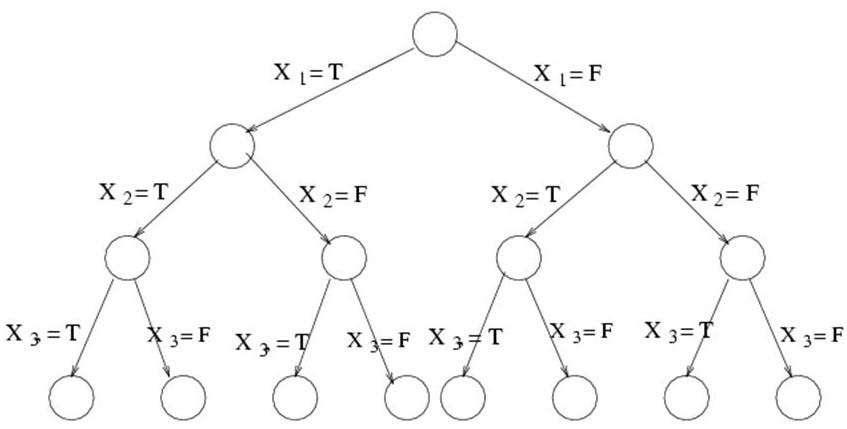
\includegraphics[width=0.7\linewidth]{images/assignment_tree.jpg}
    \caption{Esempio basilare di un albero degli assegnamenti su 3 variabili.}
    \label{fig:assignment_tree}
\end{figure}
Un approccio ingenuo al problema SAT potrebbe provare a esplorare l'albero in profondità
e restituire true se il ramo esplorato porta alla soddisfacibilità, effettuando il backtracking se la WFF si rivela insoddisfacibile per l'assegnamento associato al ramo. Ciò richiede però l'esplorazione di $O(2^n)$ rami. \\
Gli algoritmi di risoluzione basati sull'esplorazione dell'albero cercano quindi di ridurre al minimo il numero di rami esplorati e, di conseguenza, il tempo di 
esecuzione. Nel caso peggiore, però, tutti gli algoritmi conosciuti mantengono un caso peggiore di $O(2^n)$ e, quindi,
SAT rimane un problema intrattabile.\\
\\
Una delle tecniche più famose utilizzata da DPLL per migliorare l'esecuzione è la unit propagation.
Con unit clause si intende una clausola CNF contenente un solo letterale; per soddisfare la clausola, di conseguenza, è necessario
rendere vero quell'unico letterale.
Quando si presenta una unit clause all'interno di una WFF, la variabile su cui è definita deve quindi assumere valore
true se il letterale è positivo, false altrimenti.
Dopo aver effettuato l'assegnamento, tutte le clausole della WFF contenenti il letterale della unit clause possono essere rimosse,
in quanto soddisfatte proprio da quel letterale, e nelle clausole in cui invece compare il letterale opposto, esso viene semplicemente
rimosso.
Questa rimozione avviene senza problemi in clausole non ancora soddisfatte che hanno almeno due letterali. Se invece la clausola non
ancora soddisfatta da cui si deve rimuoverlo è a sua volta una unit clause, allora essa risulta non soddisfatta dall'assegnamento
corrente e, di conseguenza, non lo è tutta la WFF: bisogna quindi effettuare backtracking.\\
Se non sono presenti unit clause, l'algoritmo DPLL seleziona una variabile utilizzando delle euristiche di splitting.
Le euristiche più utilizzate sono la \textit{pure literal heuristic}, in cui viene scelta una variabile che compare nella WFF
solo col letterale positivo o solo negativo, e la \textit{most present variable}, che seleziona quella presente in più clausole.\\
Il backtracking utilizzato da DPLL è di tipo cronologico: quando un ramo dell'albero porta all'insoddisfacibilità, l'algoritmo 
effettua il backtracking fino al nodo interno più in profondità per cui sono ancora aperte delle possibili scelte.
Questo implica che, se l'insoddisfacibilità si verifica nel sottoalbero sinistro di un nodo interno, l'algoritmo passerà
a valutare il sottoalbero destro, cambiando di fatto il valore assegnato alla variabile di splitting di quel nodo.
Se invece è il sottoalbero destro a portare all'insoddisfacibilità, allora significa che qualsiasi assegnamento alla
variabile di splitting per il nodo interno non porta alla soddisfacibilità e verrà quindi restituita l'insoddisfacibilità
al nodo padre.
Lo stesso ragionamento viene applicato ricorsivamente ai nodi antenati.\\
Se è la radice ad essere il nodo interno con entrambi i sottoalberi che portano all'insoddisfacibilità, allora si può affermare 
che la WFF è insoddisfacibile.


\subsection{Algoritmo CDCL}
CDCL (Conflict-Driven Clause Learning) \cite{handbook-cdcl} è un algoritmo più moderno rispetto a DPLL (il primo articolo
è stato pubblicato nel 1996) ma ne trae molta ispirazione.
La principale differenza sta nel fatto che al verificarsi di un conflitto, ovvero quando
la WFF non risulta verificata per l'assegnamento parziale corrente, l'algoritmo apprende quali assegnamenti a quali 
particolari variabili hanno portato al conflitto e, di conseguenza, può evitarli completamente nell'esplorazione di altre parti dell'albero degli assegnamenti.\\
Questo permette, inoltre, di effettuare un \textit{backtracking non cronologico}, ovvero 
il backtracking non riprende dal nodo più in profondità con ancora scelte aperte, ma da quello
che viene ritenuto in un certo senso migliore per un eventuale scoperta di un assegnamento valido.
Molti rami dell'albero che non portano alla soddisfacibilità non vengono quindi esplorati e,
di conseguenza, i tempi di esecuzione si riducono.
Il backtracking non cronoligico di CDCL prende il nome di \textit{backjumping}.\\
\\
Per capire come funziona il backjumping è però necessario introdurre
la nozione di \textit{grafo delle implicazioni}.
Come è stato detto nella sezione relativa all'algoritmo DPLL,
quando è presente una unit clause il suo letterale deve essere obbligatoriamente soddisfatto per la soddisfacibilità della WFF.
L'assegnamento alla variabile su cui è definito però, ripercuotendosi anche sulle altre clausole,
può portare a degli assegnamenti a cascata anche su altre variabili, fino a ottenere una WFF
con meno clausole, di cui si deve continuare a verificare la soddisfacibilità, o un conflitto.\\
Questi assegnamenti a cascata possono quindi essere modellati in un grafo orientato, appunto il grafo delle
implicazioni.
Un nodo rappresenta l'assegnamento di un valore di verità a una particolare variabile.\\
Un arco orientato rappresenta invece un'implicazione: l'arco $(u, v)$ specifica che l'assegnamento
nel nodo $u$ porta obbligatoriamente all'assegnamento del nodo $v$.
Un conflitto si verifica quando, nel grafo delle implicazioni, sono presenti i due assegnamenti 
dei due valori di verità alla stessa variabile.

\begin{figure}[H]
    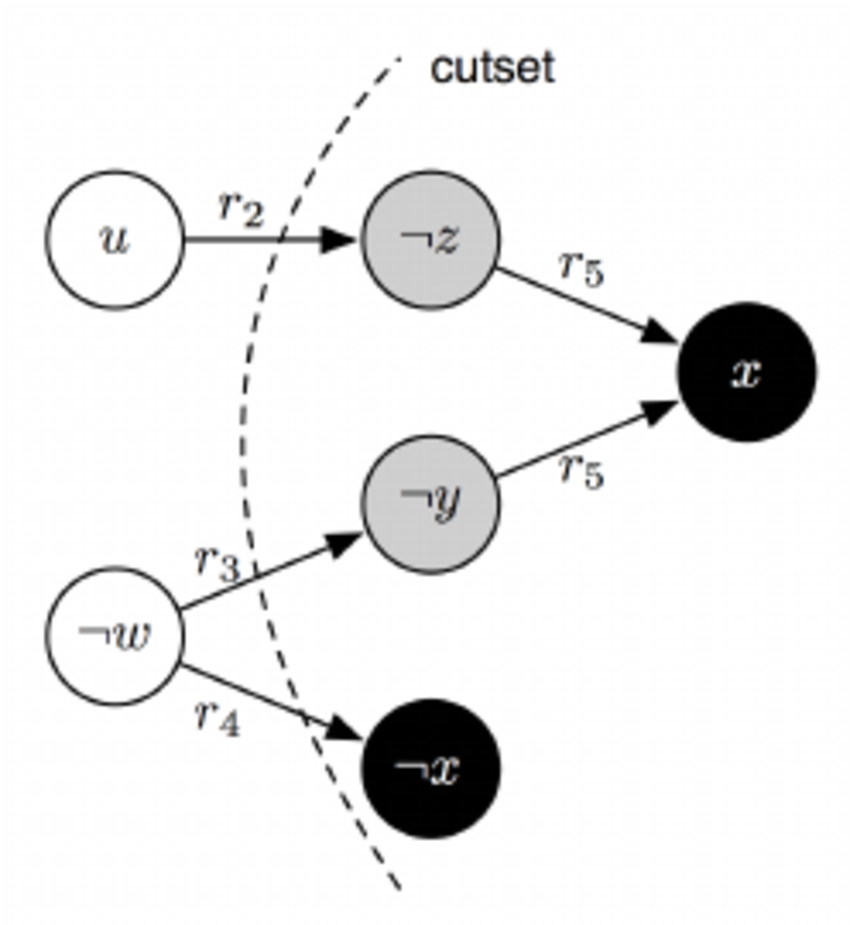
\includegraphics[scale=0.15]{images/implication_graph.png}
    \centering
    \caption{Esempio di grafo delle implicazioni e taglio su esso. \cite{implication_graph}}
    \label{fig:implication_graph}
\end{figure}

Nel caso in cui si verifichi un conflitto, sul grafo delle implicazioni può essere effettuato 
un \textit{taglio}, ovvero un partizionamento dell'insieme dei nodi
in due sottoinsiemi, in modo tale che i due nodi che hanno generato il conflitto appartengano allo 
stesso sottoinsieme e che tutti gli archi che attraversano il taglio vadano dal primo
sottoinsieme, che non contiene il conflitto, all'altro.
Si può quindi affermare che, qualsiasi sia il taglio effettuato, l'assegnamento alle variabili
del primo sottoinsieme porta necessariamente al conflitto, e deve quindi essere evitato: vengono quindi aggiunte alla WFF delle clausole che indicano che l'assegnamento parziale del primo sottoinsieme non è accettabile.\\
Una volta apprese le clausole, l'algoritmo effettua il backjumping, ovvero riprende la sua esecuzione
da un particolare livello di decisione dell'albero degli assegnamenti. In particolare,
riprende l'esecuzione dal livello che per primo ha assegnato una variabile che ha portato al conflitto,
ovvero da quello in cui è iniziata la unit propagation che si è rivelata fallimentare.\\
\\
CDCL è usato in tutti i SAT solver moderni che si basano su DPLL, come Minisat 
\cite{minisat}, Glucose e Picosat \cite{picosat-site}.

\subsection{Algoritmo di ricerca locale}
L'algoritmo di ricerca locale affronta il problema SAT in maniera differente da algoritmi come DPLL e CDCL, e non
può essere utilizzato per dimostrare la non soddisfacibilità di una WFF, ma solo una sua eventuale soddisfacibilità
\cite{local-search-no-unsat}.
Durante la sua esecuzione, infatti, modifica l'assegnamento corrente in modo tale da minimizzare il numero
di clausole non soddisfatte ed eventualmente, se un assegnamento verifica tutte le clausole, restituisce true, indicando
che la WFF è soddisfacibile.
SAT viene quindi ora trattato come un problema di ottimizzazione, in particolare di minimizzazione di una funzione che conta il numero di clausole non soddisfatte.
L'algoritmo è inoltre detto di ricerca \textit{locale} in quanto, ad un certo step, prende una decisione utilizzando
solo informazioni note a livello locale, senza considerare l'insieme globale degli assegnamenti.
A differenza di DPLL, inoltre, opera su assegnamenti completi, ovvero in cui tutte le variabili hanno assunto un valore.\\
\\
Per poter utilizzare questo algoritmo bisogna innanzitutto definire il concetto di assegnamento \textit{neighbour}:
gli assegnamenti neighbour dell'assegnamento corrente su $n$ variabili sono tutti quelli che condividono 
gli stessi valori booleani per $n-1$ variabili, mentre una variabile risulta di valore opposto.
Per ogni assegnamento su $n$ variabili, quindi, i nodi vicini sono esattamente $n$. \\
\\
Esistono molti algoritmi di ricerca locale per la risoluzione di SAT (solitamente 3-SAT), ma il più
diffuso è WalkSAT \cite{walksat-og}, utilizzato in SAT solver come UBCSAT \cite{ubcsat-site}.
Esso è in realtà una modifica di un altro algoritmo di ricerca locale greedy, chiamato GSAT:
viene infatti utilizzato un diverso criterio di cammino sugli assegnamenti, il quale permette di ridurre il numero
di assegnamenti non validi che vengono verificati; la struttura di base rimane però invariata, e per questo motivo
verrà qui analizzato l'algoritmo GSAT.
\begin{algorithm}[H]
    \caption{Pseudocodice dell'algoritmo di ricerca locale.}
    \label{algo:local_search}
    \begin{algorithmic}[1]
        \Procedure{Local-search}{wff}
            \For{i $\gets$ 1 to MAXTRIES}
                \State assg $\gets$ nuovo assegnamento casuale
                \For{j $\gets$ 1 to MAXFLIPS}
                    \If{\Call{Is-wff-satisfied}{wff, assg}}
                        \State \Return true
                    \EndIf
                    \State bestNeighbour $\gets$ \Call{Find-best-neighbour}{wff, assg}
                    \State currentUnsat $\gets$ \Call{Count-unsat-clauses}{wff, assg}
                    \State neighUnsat $\gets$ \Call{Count-unsat-clauses}{wff, bestNeighbour}
                    \If{currentUnsat $<$ neighUnsat}
                        \State \textbf{break}
                    \Else
                        \State assg $\gets$ bestNeighbour
                    \EndIf
                \EndFor
            \EndFor
            \State \Return false
        \EndProcedure
    \end{algorithmic}
\end{algorithm}
GSAT parte innanzitutto generando in maniera casuale un assegnamento:
se l'assegnamento verifica la WFF, allora si è ottenuta una soluzione ottima globale 
e la WFF è soddisfatta; se ciò non accade, l'algoritmo valuta tutti gli assegnamenti neighbour e, 
tra tutti, seleziona quello che soddisfa più clausole: 
\begin{itemize}
    \item se l'assegnamento neighbour migliore verifica più clausole dell'assegnamento corrente, allora esso viene reso corrente e l'analisi dei neighbour viene ripetuta.
    Questo spostamento a un assegnamento neighbour può avvenire al massimo MAX-FLIPS numero di volte, in modo da evitare che l'algoritmo, nel caso peggiore, esplori tutto lo spazio degli assegnamenti;
    \item se l'assegnamento neighbour migliore verifica meno clausole di quello corrente, allora la soluzione corrente
    è un ottimo locale e il ciclo interno non produce più soluzioni migliori.
\end{itemize}
Quando viene trovata una soluzione ottima locale non globale, non è detto che la WFF non abbia effettivamente
altri assegnamenti validi (e di conseguenza minimi globali): entra quindi in gioco
il ciclo esterno dell'algoritmo, che genera un nuovo assegnamento, sperando che porti all'assestamento
su un minimo globale.
La generazione casuale di un nuovo assegnamento può avvenire al massimo MAX-TRIES volte: se, al termine del ciclo
esterno, l'algoritmo non ha trovato un assegnamento valido, allora non significa obbligatoriamente che la WFF non sia soddisfacibile, ma 
semplicemente che trovarlo, se presente, richiederebbe troppo sforzo computazionale.\\
\\
WalkSAT, ovvero la variante più moderna di GSAT, è molto efficiente nella decisione della soddisfacibilità di una WFF di un problema $k$-SAT quando il rapporto
$m/n$, con $m$ numero di clausole e $n$ numero di variabili, è $m/n < c2^k/k, c > 0$ \cite{walksat-when-fast}: in questo caso, infatti, l'algoritmo riesce a trovare
un eventuale assegnamento in tempo lineare in funzione del numero di variabili $n$.
Detta transizione di fase quel valore $s$ stabilito sperimentalmente per cui $m/n < s$ implica una probabilità di soddisfaciblità tendente a 1, e $m/n > s$ implica una probabilità di soddisfacibilità tendente a 0; l'utilizzo di WalkSat è sconsigliato quando $m/n$ è leggermente maggiore della transizione di fase: in questo caso, infatti, i pochi eventuali 
assegnamenti che soddisfano la WFF si organizzano in piccoli cluster 
di assegnamenti neighbour validi, separati però da numerosi assegnamenti che non soddisfano la WFF. 
Di conseguenza, un algoritmo come WalkSAT o si assesta su minimi 
locali, che quindi non sono soluzioni del problema, o la generazione di un assegnamento casuale, usata
proprio per evitare di assestarsi su dei minimi locali, ha poca probabilità di generare un assegnamento
che porti a un'eventuale soluzione della WFF \cite{walksat-fails}.\\
\\
A partire dal 2013, i SAT solver basati su ricerca locale sono stati superati da quelli
basati su CDCL con preprocessing, e non sono quindi attualmente i più performanti \cite{handbook-preprocessing}. 